\let\negmedspace\undefined
\let\negthickspace\undefined
\documentclass[journal]{IEEEtran}
\usepackage[a5paper, margin=10mm, onecolumn]{geometry}
%\usepackage{lmodern} % Ensure lmodern is loaded for pdflatex
\usepackage{tfrupee} % Include tfrupee package

\setlength{\headheight}{1cm} % Set the height of the header box
\setlength{\headsep}{0mm}     % Set the distance between the header box and the top of the text

\usepackage{gvv-book}
\usepackage{gvv}
\usepackage{cite}
\usepackage{amsmath,amssymb,amsfonts,amsthm}
\usepackage{algorithmic}
\usepackage{graphicx}
\usepackage{textcomp}
\usepackage{xcolor}
\usepackage{txfonts}
\usepackage{listings}
\usepackage{enumitem}
\usepackage{mathtools}
\usepackage{gensymb}
\usepackage{comment}
\usepackage[breaklinks=true]{hyperref}
\usepackage{tkz-euclide} 
\usepackage{listings}
% \usepackage{gvv}                                        
\def\inputGnumericTable{}                                 
\usepackage[latin1]{inputenc}                                
\usepackage{color}                                            
\usepackage{array}                                            
\usepackage{longtable}                                       
\usepackage{calc}                                             
\usepackage{multirow}                                         
\usepackage{hhline}                                           
\usepackage{ifthen}                                           
\usepackage{lscape}
\begin{document}

\bibliographystyle{IEEEtran}
\vspace{3cm}

\title{9.1.10}
\author{EE24BTECH11009 - Mokshith Kumar}
\maketitle

\textbf{Question:}\\
Solving the second-order differential equation:
\begin{align}
y'' + 2y' + \sin{y} = 0
\end{align}
\textbf{Solution:}\\
An exact theoretical solution using known methods to solve differential equations was not found. Therefore, we will use the numerical method(Euler method) to approximate the solution.\\

To apply the Euler method, we first need to convert the second-order differential equation into a system of first-order differential equations.

Let:
\begin{align}
v = y' \quad \text{(first derivative of \( y \))}\\
\end{align}
Then
\begin{align}
v' = y'' \quad \text{(second derivative of \( y \))}
\end{align}
Substitute \( y' = v \) into the original differential equation:
\begin{align}
v' + 2v + \sin(y) = 0
\end{align}
This simplifies to the following system of first-order equations:
\begin{align}
\frac{dy}{dx} = v\\
\frac{dv}{dx} = -2v - \sin(y)
\end{align}
Thus, we now have the system:
\begin{align}
\frac{dy}{dx} = v
\frac{dv}{dx} = -2v - \sin(y)
\end{align}
For each step, Euler's method updates the solution using the following formulas:

\begin{align}
    y_{n+1} = y_n + h \cdot v_n\\
    v_{n+1} = v_n + h \cdot (-2v_n - \sin(y_n))\\
    x_{n+1}=x_{n}+h
\end{align}
\\Where $ y_n$ and $v_n$ are the values of $y$ and $v$ at the $n$-th step,$h$ is the step size (which controls the accuracy of the method),
$y_{n+1}$ and $v_{n+1}$ are the updated values for the next step.\\
Now, consider the initial conditions as
$\\x_0=0.0\\y_0=1.0\\v_0=1.0\\h=0.01\\$
The following plot is obtained.
\begin{figure}[h!]
   \centering
   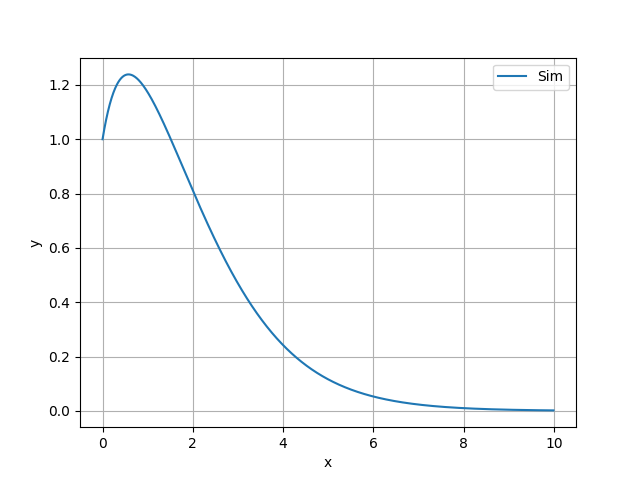
\includegraphics[width=\columnwidth]{figs/9.1.10.png}
   \caption{Plot of the computational solution of $y'' + 2y' + \sin(y) = 0$.}
   \label{}
\end{figure}
\end{document}

